\documentclass{aa}
\usepackage[varg]{txfonts}
\usepackage{graphicx}       % Include figure files
\usepackage{amsfonts,amsmath}
\usepackage{natbib}
\usepackage{color}
%%%%%%%%%%%%%%%%%%%%%%%%%%%%%%%%%%%%%%%%%%%%%%
% Sarp's commands
\newcommand{\be}{\begin{equation}}
\newcommand{\ee}{\end{equation}}
\newcommand{\f}{\frac}
\newcommand{\nn}{\nonumber}
\newcommand{\ord}{\mathcal{O}}
\newcommand\T{\rule{0pt}{2.6ex}}       % Top strut for vertical spacing in tables
\newcommand\B{\rule[-1.2ex]{0pt}{0pt}} % Bottom strut
\newcommand{\M}{\mathcal{M}_c}
\newcommand{\sa}[1]{{\textcolor{red}{\texttt{SA: #1}} }}
\newcommand{\mf}[1]{{\textcolor{magenta}{\texttt{MF: #1}} }}
\newcommand{\ac}[1]{{\textcolor{orange}{\texttt{AC: #1}} }}

%%%%%%%%%%%%%%%%%%%%%%%%%%%%%%%%%%%%%%%%%%%%%%
%%%%%%%%%%%%%%%
%%%%%%%%
%%%
%
\begin{document}
\title{
%Forecasting Gamma-Ray Bursts with Gravitational-wave Detectors
%Electromagnetic follow-ups in the era of forecasting gamma-ray bursts
%\thanks{Grant1}\fnmsep
%\thanks{Grant2}\\
A crystal ball for kilonovae
}
%\subtitle{Early warnings for Gravitational Waves from the Einstein Telescope}
\subtitle{Early warnings from Einstein Telescope for electromagnetic follow-ups}
\author{Sarp Akcay\inst{1}\inst{2}
\and Morgan Fraser\inst{3}
\and Antonio Martin-Carrillo\inst{3}}
%\thanks{\emph{Present address:}
%Department of Computer Science, Purdue University,
%West Lafayette, IN 47907, USA}

\institute{Theoretisch-Physikalisches Institut, Friedrich-Schiller-Universit{\"a}t, 07743, Jena, Germany
\and School of Mathematics \& Statistics, University College Dublin, Belfield, Dublin 4, Ireland
\and School of Physics, University College Dublin, Belfield, Dublin 4, Ireland} % Space Science Group,
% \date{Received 2 November 2018 / Acecpted 7 January 2018}
\abstract{
The discovery of gravitational waves from merging compact objects has opened up a new window to the Universe. Planned third-generation gravitational-wave detectors such as Einstein Telescope will potentially deliver hundreds of such events at redshifts below $z\sim0.1$. Finding electromagnetic counterparts to these events will be a major observational challenge. We demonstrate how Einstein Telescope will provide advance warning of 
such events on a timescale of hours, based on the low frequency emission from the pre-merger system. In addition, we suggest how this early warning enables prompt identification of any electromagnetic counterpart using the Large Synoptic Survey Telescope.
%detection of gravitational waves from the binary neutron star inspiral-merger event GW170817 and the subsequent
%extended electromagnetic follow-up observations of the resulting kilonova
%gave us a small taste of multi-messenger astronomy across the spectra of \emph{two} fundamentally
%different kinds of radiation.
%The opportunities to conduct such multi-disciplinary studies will increase by two orders of magnitude
%in the 2030s with Einstein Telescope (ET), LIGO's European successor.
%Due to its extreme sensitivity in the $1-10\,$Hz regime, the Einstein Telescope's C configuration (ET-C) will be capable of detecting inspiralling binary neutron star systems out to luminosity distances of 1 Gpc.
%Within half of this distance, 
%-to-noise ratios of $\gtrsim 15$ %and localize the source to $\lesssim \mathcal{O}(10)\,\text{deg}^2$ 
%ET is expected to anually localise $\gtrsim 5 $ binary neutron stars to $\Delta\Omega\lesssim 10\,$deg$^2$ with $\gtrsim$ one hour left to merger.
%This yearly rate can potentially quadruple with the inclusion of a second detector like
%Cosmic Explorer, the proposed third generation US detector. There will additionally be up to $\mathcal{O}(100)$ sources
%with $\Delta\Omega\sim 20\,$deg$^2$.
%
%On the other hand, a second less sensitive gravitational-wave detector (such as future KAGRA)
%GW detector with just ten times KAGRA sensitivity at 5\,Hz 
%would increase the number of well-localized sources to $\mathcal{O}(100)$.
%Thus it is imperative to have at least one companion detector to ET with significantly improved seismic isolation in the 2030s.
%Having so many ``well'' localised GW sources opens the possibility of doing detailed follow-up observations of
%the resulting kilonovae with the next generation electromagnetic observatories such as the LSST.
%Here we explore this intriguing possibility...\\
%Here, we investigate the potential issues in the follow-up work such SNIa posing as kilonovae in the optical band.
%Thus, this letter is an appeal/plea(?) to the astronomy community to have in place ...
%We explore the  possibility of employing future ground-based gravitational-wave interferometers to detect the inspiral of binary neutron stars sufficiently
%early to alert electromagnetic observatories so that a gamma-ray burst (GRB) can be observed in its entirety from its very beginning.
%We quantify the ability to predict a GRB by computing the time a binary neutron star (BNS) system takes to inspiral from its moment of detection to its final merger. We define the moment of detection to be the instant at which the inteferometer network accumulates a signal-to-noise ratio of 15. %for the BNS inspiral.
%For our computations, %of advance warning times, 
%we specifically consider BNS systems at luminosity distances of (i) $D\le200\,$Mpc in the three-interferometer Advanced-LIGO-Virgo network of 2020, and (ii) $D \le 1000\,$Mpc in the Einstein Telescope's B and C configurations. 
%In the case of Advanced LIGO-Virgo we find that we may at best get a few minutes of warning time, thus we expect no forecast of GRBs in the 2020s. 
%On the other hand, Einstein Telescope will provide us with advance warning times of more than five hours for $D \le 100\,$Mpc.
%Taking one hour as a benchmark advance warning time, we obtain a corresponding horizon
%distance of roughly 600 Mpc for the Einstein Telescope C configuration.
%Using current BNS merger event rates within this volume, we show that Einstein C will forecast $\gtrsim \mathcal{O}(10^2)$ GRBs in the 2030s. %with Einstein C. %with the C configuration of Einstein Telescope.
%We reapply our warning-time computation to binary black hole - neutron star inspirals and find that we expect 1 to 3 tidal disruption events to be forecast by the same detector.
}
\keywords{gravitational waves --gamma-ray bursts -- kilonovae}
\maketitle

\section{Introduction}

%Gravitational waves offer a unique insight into some of the most extreme physical processes in the Universe - including the merger of black holes (BH) and neutron stars (NS), and the first seconds of core-collapse supernovae (SNe) explosions. 
With the first direct detection of gravitational waves (GWs) in 2015 by the Advanced Laser Interferometer Gravitational-Wave
Observatory (Advanced LIGO; \citealp{FirstGW}), gravitational-wave astronomy moved from prospect to reality. The first GW source observed by Advanced LIGO, GW150914, matched the signal predicted for the merger of two black holes with masses 36 and 29 M$_{\odot}$.
%Along with being the first direct detection of GWs, GW150914 was also the first detection of such heavy black holes, which had significantly larger masses compared to those measured for galactic high mass X-ray binaries. Such massive black holes provide an interesting constraint on stellar evolutionary channels at low metallicity \citep[e.g.][]{FirstGW_astro, Belc16}. While no electromagnetic counterpart is generally expected to accompany the merger of two black holes, an intensive multi-wavelength search of the probable location of GW150914 was carried out \citep{FirstGW_EM}. Despite yielding a null result, this effort served as a rehearsal in preparation for searches for counterparts to GW sources that {\it are} expected to be accompanied by an electromagnetic (EM) source.

Only two years after GW15014, %the first detection of merging black holes, 
the Advanced LIGO and Virgo gravitational-wave observatories detected GW170817, with a waveform consistent with the merger of two neutron stars \citep{GW170817}. A spatially and temporally coincident short Gamma Ray Burst (GRB) was also seen by the {\it Fermi} and {\it INTEGRAL} satellites \citep{GW170817_GRB}. This discovery sparked a global effort to find the counterpart of GW170817 at optical wavelengths, which resulted in the identification of AT2017gfo less than 11 hours later \citep{GW170817_EM}. AT2017gfo faded exceptionally rapidly, and displayed cool temperatures and lines from unusual r-process elements at exceptionally high velocities \citep{Smar17,Arca17,Pian17,Coul17,Kilp17}. These characteristics marked AT2017gfo as a kilonova; a transient powered by the radioactive decay of short-lived nuclides formed in the merger of two neutron stars.

The detection of electromagnetic (EM) counterparts to GWs from merging neutron stars is of exceptional significance for astrophysics. Kilonovae are the predominant site for r-process nucleosynthesis, and so play a critical role in the chemical evolution of galaxies. If a kilonova can be identified and associated with a host galaxy of known redshift, then the degeneracy between inclination angle and distance inherent to a GW signal can be broken. This in turn allows the opening angle of the GRB jet to be constrained, something that has been done for a handful of GRBs to date \citep{2018ApJ...857..128J}. GW %Gravitational wave 
sources can also be used to independently determine the Hubble constant $H_0$ \citep{GWH0}.
%This of particular interest given the disagreement between measurements of $H_0$ from Type Ia SNe and from the Cosmic Microwave Background \citep[e.g.,][]{Bern16}

The identification of AT2017gfo as the counterpart to GW170817 was realised by the 
ability of Advanced LIGO-Virgo to localise the GW signal to $\sim30~\mathrm{deg}^2$.
%small region on the sky ($\sim$30 deg$^2$) within which the GW was localised. 
In addition, at only 40 Mpc, GW170817 was exceptionally close. This enabled the EM counterpart to be identified through targeted observations of galaxies at this distance within the GW localisation region \citep{Coul17}. Unfortunately, such a strategy is only feasible for the nearest GW sources, and rapidly becomes irrealisable beyond $\sim100$ - $200$ Mpc, both as the number of galaxies within the search volume increases, and as the fraction of galaxies with reliable redshifts decreases. 
This embarrassment of riches is a serious obstacle for identifying EM counterparts to GW transients that will be detected by Einstein Telescope in the 2030s \citep{ET_doc}.

%Einstein Telescope (ET) will be sensitive enough to ``pick up'' GW sources at a few Hz thanks to
%its cryogenic design and underground housing which will shield it from low-frequency contaminants such as seismic and gravity-gradient noises. Moreover, 
 Einstein Telescope (ET) will consist of three
 V-shaped interferometers which eliminate blind spots and further allow it to construct a null
 stream \citep{Sathyaprakash:2012jk} which can be used to veto spurious events \citep{Wen:2005ui}. 
 Additionally, ET will be a xylophone \citep{Hild:2009ns}, i.e., a multi-band detector capable of delivering high sensitivities both at low frequencies ($\sim 5\,$Hz) and high frequencies ($\sim 100\,$Hz). 
 %as we show in .
 Here, we focus on the C configuration (ET-C) which offers the highest low-frequency sensitivity as shown in Fig.~\ref{fig:ETB2030}.
 ET-C will detect $\gtrsim\mathcal{O}(10^3)$ binary neutron star inspirals per year out to 1~Gpc \citep{Akcay18}.  %with SNRs $\gtrsim 30 $ \citep{Akcay18}. 
 A subset of these sources will be close enough that they will be detected a few hours
before their respective mergers \citep{Akcay18}, hence opening up the possibility of alerting EM
observatories to conduct follow-up observations \emph{before, during} and after the prompt gamma-ray burst. 
Additionally, ET-C will yearly forecast a few tidal disruption events from NS - BH (black hole) binaries \citep{Akcay18}.
%in which a neutron star gets tidally torn by a $\sim 5 M_\odot$, high-spin black hole companion 
%{\bf Morgan:} should we add more details here such as specific numbers for events/year? I was
%leaving these for Sect. 2

%{\bf Something on future GW observatories - introduce Einstein Telescope etc. How many events do we expect to see per year? What at the timescales for these coming online}

To fully exploit the prospect of multi-messenger astronomy, a number of wide-field survey telescopes are either operational, in commissioning, or under construction. Foremost among these is the Large Synoptic Survey Telescope \citep[LSST;][]{LSSTbook}, which has an 8.4\,m primary mirror, and will image $9.6~\mathrm{deg}^2$ in a single pointing. Construction of LSST is well underway
with full survey operations starting in 2023.
%and the telescope is expected to begin full survey operations at the start of 2023. 
Apart from LSST, the majority of current and next-generation survey telescopes have a relatively small mirror, but a large camera, and are designed to observe $\sim10-50~\mathrm{deg}^2$ in a single pointing to a limiting magnitude of $\sim20$ - $22$. ZTF \citep{ZTF}, GOTO \citep{GOTO} and ATLAS \citep{ATLAS} are all currently operational, while BlackGEM is under construction \citep{BlackGEM}.

There has been a considerable amount of discussion in the literature as to the optimal strategy to identify an EM counterpart to future GW transients \citep{2016ApJ...820..136G, 2011MNRAS.415L..26C, 2016A&A...592A..82G, 2017ApJ...834...84C, 2014MNRAS.437..649S, 2016MNRAS.462.1085A, 2018arXiv181204051M}. In most cases however, a large number of candidates will be found within the search region, for which further spectroscopic follow-up observations will be required. This spectroscopic classification bottleneck will remain a problem into the foreseeable future.

%{\bf Intro to rest of paper. Our novel contribution is that we get an early warning for GWs. Can then use this to get templates immediately prior to the GW detection. Outline rest of section.}

Our aim here is to demonstrate exciting EM follow-up studies that can be done by taking advantage of the early GW warning capability of ET. 
The ability of ET to detect inspiraling compact objects $\sim$hours before the merger has been described in detail by \cite{Akcay18}, and in this Letter we 
present a brief summary of these results and their implications for follow-up observations of electromagnetic counterparts.
%We
%consider binary neutron star inspirals
%out to luminosity distances of $\sim 600\,$Mpc, 
%the expected range of LSST. Within this range,
%ET-C will be able to detect GWs from inspirals
%a few hours before a given merger thus provide
%a window of opportunity for mobilizing the EM
%observatories in time to witness the birth of 
%the associated kilonova. Furthermore, a pre-GRB GW warning allows us to 
%obtain reference images with EM telescopes immediately prior to a kilonova, reducing the number
%of unrelated transients that will be found within a given search region.
%However, in order to
%fully benefit from ET's early warnings, several
%issues must be addressed: (i) ET's poor localisation by itself, (ii) large number of 
%supernovae creating a confusion background, 
%(iii) the slow response time of certain EM 
%observatories essential to follow-up. % such as ATHENA, BLACKGEM {\bf Antonio, Morgan, is this right?}
%Here, we consider each of these setbacks and
%suggest solutions which require support from the global astronomy community.

%This letter is organized as follows: Sect.~\ref{sect:et} provides more details on ET,
%Sect.~\ref{sect:EM} investigates the implications
%of optical follow-up. %Sect.~4 ...
We use $f$ to denote the quadrupole GW frequency
in the detector frame. $G$ is Newton's constant and $c$ is the speed of light.


\section{Einstein Telescope}
\label{sect:et}
In this section, we compute the advance warning times ($T_\text{AW}$) ET will provide (computational details are provided in \cite{Akcay18}).
%To this end, 
Consider a binary neutron star (BNS) system with component masses
$m_1, m_2$ inspiraling at a luminosity distance $D$ with a corresponding redshift $z$. For GW frequencies of interest here ($f \lesssim 10\,$Hz), the binary undergoes an adiabatic inspiral dominated by
the emission of leading-order (quadrupole)
gravitational radiation. By balancing the
power emission in GWs to the rate of change of binding energy, we obtain the frequency evolution of the GW frequency
%
\be
\dot{f} = \f{96}{5}\pi^{8/3} \f{(G \mathcal{M}_c)}{c^5}^{5/3}\, f^{11/3}, \label{eq:fdot}
\ee
where $\mathcal{M}_c  = (1+z){(m_1 m_2)^{3/5}}{(m_1+m_2)^{-1/5}}$ is the redshifted chirp mass. 
%with $M_c={(m_1 m_2)^{3/5}}{(m_1+m_2)^{-1/5}} $.
After fixing the integration constant, Eq.~(\ref{eq:fdot})
can be integrated to yield the time left to merger at a given frequency, usually called the inspiral time
%
\begin{align}
\tau_\text{insp}(f) &= \f{5}{256\pi}\f{c^5}{(\pi G \M)^{5/3}} \,f^{-8/3}\nn\\
&=16.72\,\text{minutes} \, \left(\f{1.219 M_\odot}{\M}\right)^{5/3}\,\left(\f{10\,\text{Hz}}{f}\right)^{8/3}
\label{eq:tau_insp}\, .
\end{align}
%
This result can be supplemented with a post-Newtonian series up to $\ord(c^{-2})$ \citep{Blanchet_LRR}, but the resulting expressions
 only change $\tau_\text{insp}$ by $\lesssim 2\%$.

%To obtain $T_\text{AW}$ we must choose a value of $f$.
%It is a well known result in general relativity that 
A passing GW induces a response in a given interferometer (IFO) known as the GW strain. %which is a function of source inclination, GW polarization, and the IFO antenna pattern. 
In frequency domain, the norm of the GW strain is given by
%
$|\tilde{h}(f)|=A h_0 f^{-7/6} |Q|,$ %\label{eq:h_tilde}
%\ee
%
where $A= \pi^{-2/3}(5/24)^{1/2},\, h_0 = c  (1+z)^{-1}\tilde{M}^{5/6}/D$ with $\tilde{M}= G \M c^{-3}$ and $Q$ is the IFO quality factor which is a function of source sky location and inclination angles $\{\theta,\phi, \iota\}$, and the relative detector-source polarization angle $\psi$.

The IFO response to a GW strain is quantified in terms of a signal-to-noise ratio (SNR).
As we can not a priori know the angles $\{\theta,\phi,\iota,\psi\}$, we use an angle-RMS-averaged SNR, 
appropriate for a detector with triangular topology like ET
%
\be
\rho_{\text{ET}}(f_1,f_2) = \frac{3}{5}\,2 A\, h_0  (1+z)^{-1/6} \left[\int_{f_1}^{f_2} d f'\, \f{f'^{-7/3}}{S_{n}(f')}\right]^{1/2} \label{eq:ET_SNR},
\ee
%
where %$z$ is the source redshift and
$\sqrt{S_n(f)}$ is the {\it amplitude spectral density} of the detector (also called detector noise) and
the factor of $3/5$ in Eq.~(\ref{eq:ET_SNR})
is due to RMS-averaging \citep{Akcay18}. %over the angles $\{\theta,\phi,\iota,\psi\}$. 
For a given source, $\rho_\text{ET}$ may vary by $\sim \pm 30\%$ compared to the average (\ref{eq:ET_SNR}), but will always be $>0$ because of ET's all-sky coverage.

%We now use Eq.~(\ref{eq:ET_SNR}) to provide a precise definition %of the advance warning time 
We define $T_\text{AW}$ as the time left to merger from the moment of detection 
%therefore we must first define the former.
%We do this using Eq.~(\ref{eq:ET_SNR}) 
defined as follows: let $f_0$ be the frequency
at which the GW strain equals the RMS-averaged detector noise, i.e., $\tfrac{5}{3}\sqrt{S_n(f_0)}=2\sqrt{f_0} \tilde{H}_\text{ET}(f_0)$ where $\tilde{H}_\text{ET}(f)= h_0 f^{-7/6}$;
the instant of detection is given by 
$\bar{f}>f_0$ such that $\rho_\text{ET}(f_0,\bar{f})=15$. 
Thus $T_\text{AW} = \tau_\text{insp}(\bar{f})$.
The total accumulated SNR is given by $\rho_\text{tot}=\rho_\text{ET}(f_0, f_\text{ISCO})$, 
where $f_\text{ISCO}$ is the frequency at which the inspiral transitions to plunge. 
Here, we use the standard approximation from general relativity: 
$f_\text{ISCO} \approx {c^3}\left[{6^{3/2}\pi\, G (m_1+m_2)(1+z)}\right]^{-1} \simeq {1571}(1-z) \left(\frac{2.8M_\odot}{m_1+m_2}\right)\text{Hz}$ for $z\ll 1$. 
We chose a conservative threshold SNR of 15. % is not set in stone;
%other common choices are 8 and 12, but we choose to be more conservative.

%The only free variable left to determine
%$T_\text{AW}$ is the luminosity distance D. % ($z$ is obtained from it and vice versa).
$D$ now fully determines $T_\text{AW}$.
In Fig.~\ref{fig:ETB2030} we display the GW strain for four canonical ($m_1=m_2=1.4 M_\odot$) BNS inspirals at $D=100,200, 400, 600\,$Mpc, 
compared to the expected ET-C sensitivity.
%ET-C's noise is the thick, red curve. % with the best sensitivity for $f\lesssim 10\,$Hz. 
%In traditional amplitude spectral density plots, 
Note that the inspiral GW strains scale as $ \sqrt{f} f^{-7/6} = f^{-2/3}$ \citep{Colpi_Sesana},
hence are straight lines with slope $=-2/3$. %in the figure.
The frequencies $f_0$, at which each inspiral enters ET-C's sensitivity band, are the intersection
points between these straight lines and the ET-C noise and lie within 1 - 2\,Hz.
We list the advance warning times along with the total SNRs for these sources in  Table~\ref{table:ET}, where
we show that ET-C is capable of providing up to \emph{five} hours of early warning before a  merger.
%
%thus offering a tremendous opportunity to electromagnetically observe the merger-GRB-kilonova with available
%resources in the 2030s.
%But we should first see if ET can forecast enough BNS events and localise them to make a follow-up campaign worthwhile.

%
%
%
%
\begin{table}[h]
\caption{Forecasting capabilities of the C configuration of Einstein Telescope. 
$D$ is the luminosity distance and $z$ the corresponding redshift 
computed assuming a flat $\Lambda$CDM universe with $\Omega_\Lambda = 0.6911, \Omega_m = 0.3089, H_0 = 67.74~\mathrm{km}~\mathrm{s}^{-1}~\mathrm{Mpc}^{-1}$ \citep{Planck2015}.
%We only present the results using the post-Newtonian enhanced version of \citep{Blanchet_LRR}
$\bar{f}$ is the threshold frequency at which ET-C accumulates SNR of 15.
$T_\text{AW}\equiv \tau_\text{insp}(\bar{f})$ [see Eq.~(\ref{eq:tau_insp})].
%is the inspiral time from the instant when the GW frequency equals $\bar{f}$.
$\rho_\text{tot}$ is the total SNR for each inspiral.
Last column lists the event rates %in the format $\text{average}^\text{max}_\text{min}$ 
%in units of $\text{yr}^{-1}$ 
within concentric shells of radius $D$ and thickness 100\,Mpc.}
%The numbers have been rounded when appropriate.}
\label{table:ET}
\centering
\begin{tabular}{lccccc}
%toprule
\hline\hline
$D\,$(Mpc) &  $z$ & $\bar{f}\,$(Hz) &  $T_\text{AW}\,$(hrs)& ${\rho}_\text{tot}$ &$ R\,(\text{yr}^{-1})$ \T\B \\
\hline
100 & $ 0.022$ & 3.3 & 5.3 & 365 & $1.54^{\,+3.20}_{\,-1.22}$ \T \B \\
200 & $ 0.044$ & 4.1 & 2.9 & 182 & $10.8^{\,+22.4}_{\,-8.54}$ \T \B \\
300 & $ 0.065$ & 4.66 & 1.9 & 121 & $29.3^{\,+60.8}_{\,-23.2}$ \T \B \\
400 & $ 0.085$ & 5.1 & 1.5 & 90.5 & $57.0^{\,+118}_{\,-45.1}$ \T \B \\
500 & $ 0.10$ & 5.4 & 1.2 & 72.2 & $93.9^{\,+195}_{\,-74.4}$ \T \B \\
600 & $ 0.12$ & 5.7 & 1.03 & 60.0 & $140^{\,+291}_{\,-111}$ \T \B \\
%100 & $ 0.022$ & 3.3 & 5.3 & 365 & $1.54^{\,4.7}_{\,0.32}$\T\B \\
%200 & $ 0.044$ & 4.1 & 2.9 & 182 & $12.3^{\,38.}_{\,2.6}$ \T \B \\
%300 & $ 0.065$ & 4.66 & 1.9 & 121 & $41.6^{\,130}_{\,8.6}$ \T \B \\
%400 & $ 0.085$ & 5.1 & 1.5 & 90.5 & $98.6^{\,300}_{\,20}$ \T \B \\
%500 & $ 0.10$ & 5.4 & 1.2 & 72 & $193^{\,590}_{\,40}$ \T \B \\
%600 & $ 0.12$ & 5.7 & 1.03 & 60 & $333^{\,1020}_{\,69}$ \T \B \\
\hline\hline
\end{tabular}
\end{table}
%
%
%
%
%
%
% Newest event rate: $R = 1210^{+3220}_{-1040}$ from 1811.12907 for Gaussian NS mass distribution 
%110 - 3840 per GPC^{-3}/yr page 27
%
\subsection{Event rates for binary neutron star inspirals}
We base our event rate calculations on $R=1540^{+3200}_{-1220}\,\text{Gpc}^{-3}\,\text{yr}^{-1}$ inferred from GW170817 \citep{GW170817} consistent with $110 - 3840~\mathrm{Gpc}^{-3}\,\text{yr}^{-1}$ \citep{LIGOScientific:2018mvr}. %Assuming flat spatial geometry, 
This translates roughly to $R(D\le 600\,\text{Mpc})=330^{+690}_{-260}~\mathrm{yr}^{-1}$. %BNS events per year within 600\,Mpc. 
We partition this volume into concentric shells each 100 Mpc thick. For each shell, we show the event rates in Table~\ref{table:ET}. %along with the corrsponding redshift assuming
%each distance computed using a flat $\Lambda$CDM model ($\Omega_k=0$) with the latest Planck satellite parameters: 
% with negligible ra yielding and $\Omega_r \lesssim 10^{-4}$.
%It is then straightforward to translate $D$ to $z$ [cf. \cite{Hogg:1999ad}].
%
%
%
%
\begin{figure*}
\sidecaption
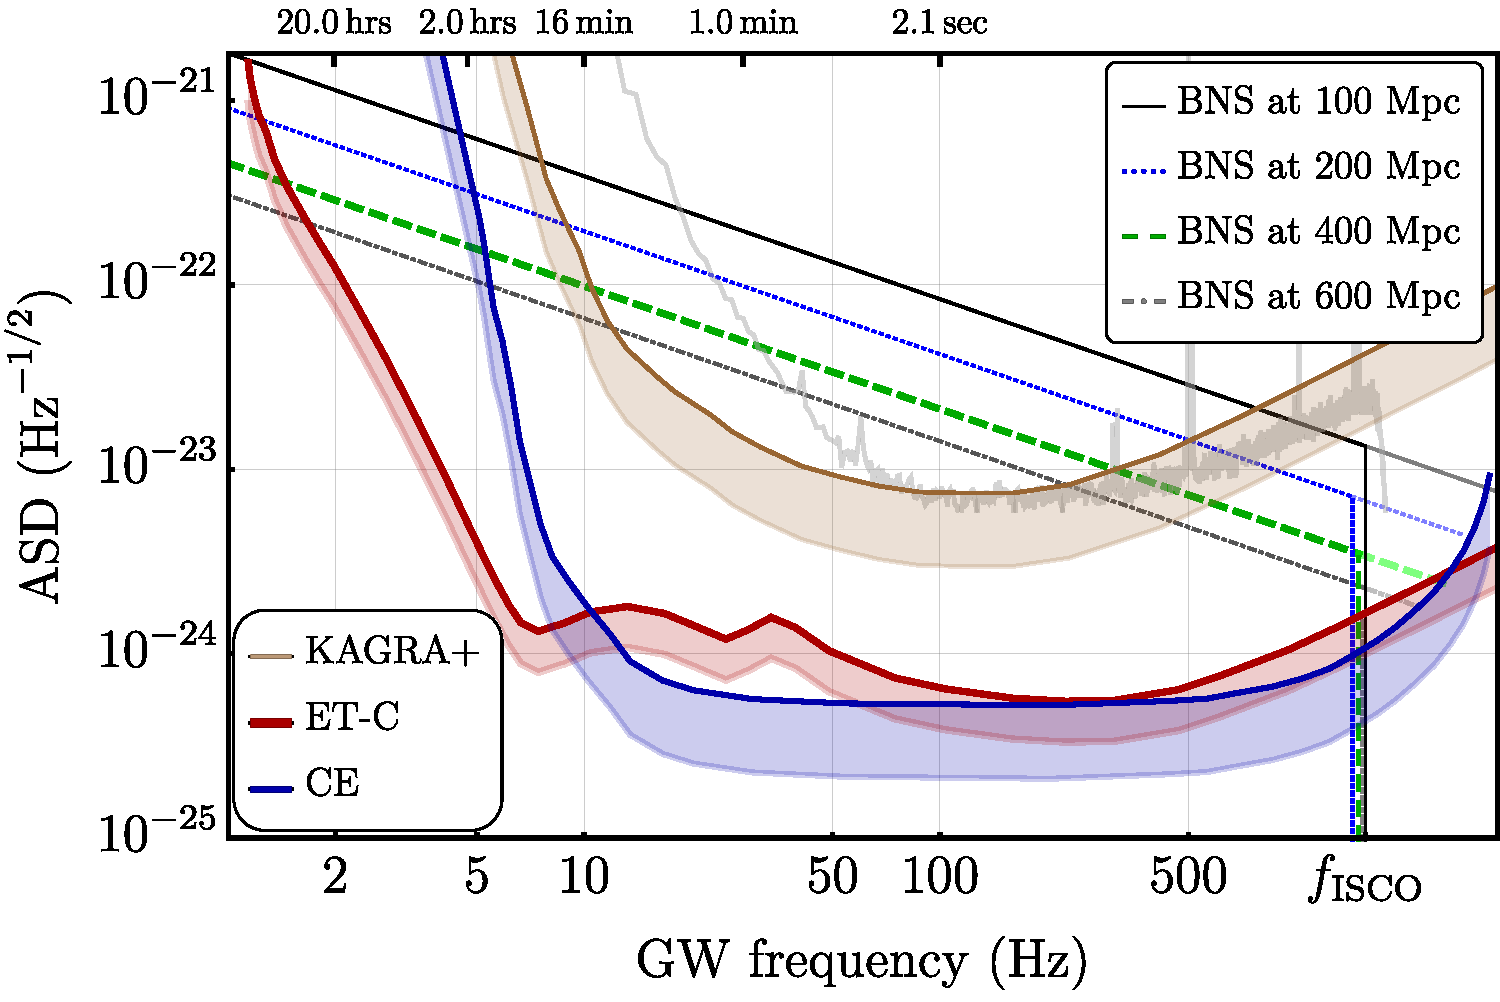
\includegraphics[width=12cm]{../Figs/ET_strains_redshifted_v4.pdf}
\caption{%Typical GW sources that may be harbingers of GRBs in the 2030s: 
$1.4 M_\sun$ - $1.4 M_\sun$ inspiralling BNS systems sweeping across the sensitivity band of Einstein Telescope's C configuration (thick red curve).
The solid (black), dotted (blue), dashed (green), and dot-dashed lines (gray) lines are the redshift-corrected GW strains, $2\sqrt{f}\tilde{H}_\text{ET}$, at luminosity distances of $D=100, 200, 400, 600\,$Mpc, respectively. 
The vertical lines with correspondingly identical patterns (colors) mark the redshifted ISCO frequencies $(1+z)^{-1} f_\text{ISCO}$ at which point we terminate each inspiral.
As the true ISCO frequency is likely larger than $f_\text{ISCO}$ \citep{Marronetti:2003hx}, the inspirals would continue to nearly 2\,kHz indicated by the faded lines in the plot.
We also show the sensitivity curves for Cosmic Explorer (blue) and KAGRA+ (brown) with the solid curves representing their RMS-averaged sensitivities and the bottom of each shaded region, the maximum sensitivities.
The faint gray curve represents the sensitivity of Advanced LIGO during GW170817.
The upper  horizontal axis gives the time to merger for a BNS at 100 Mpc.
%As the angle-RMS average for an L-topology detector is 2/3 of ET's \citep{Akcay18}, we rescale the CE, KAGRA+, LIGO curves by $3/2$. %thus making them effectively less sensitive.
%Otherwise, we would have to draw four additional BNS strains, each of which scaled down by $2/3$ in amplitude.
}
\label{fig:ETB2030}
\end{figure*}
%
%
%

We see from Table~\ref{table:ET} that %an event as near as GW170817 is a once-per-decade occurence, but
within $z\lesssim 0.1$, %we can expect 
ET-C will annually detect GWs from $\sim$ 40 to 600 BNS transients.
Roughly 7\% of these will be within 200\,Mpc yielding $T_\text{AW}\gtrsim 3\,$hours which means that EM observatories will be alerted $\sim 3$ - 40 times yearly with the prospect of observing births of kilonovae.
If we assume that future EM observatories could respond with $T_\text{AW}=1\,$hour warning, then
all BNS transients within 600\,Mpc become possible candidates for merger-kilonovae observations.
In this case, early warnings would be sent by ET at least once a week and at most three times per day.
%It is not feasible to have a system in place to observe each one of these events
%so it will make sense to be selective and focus on the best candidates.
%These  will naturally mostly be the nearest sources which will additionally be favoured by ET because of its limitations with localisation that we discuss next.
%will act as an extra selection filter, favouring events with the largest $T_\text{AW}$.

\subsection{Source localisation estimations}
%Though ET will have no blind spots because it consists of three V-IFOs in one plane, each rotated by $120^\circ$,
ET will have poor source localisation because all three of its IFOs will be co-located. 
However, as ET-C will
detect BNS inspirals hours before the merger, during this time the Earth will have rotated by $\sim 10^\circ$ - $50^\circ$.
%as much asa few dozen degrees. %This means that over this time ET can be treated as a network.
Therefore, within 1Gpc, ET \emph{alone} will localise  $\sim20$\% of sources to within $100~\mathrm{deg}^2$, 
2\% to within $20~\mathrm{deg}^2$, and 0.5\% to within $10~\mathrm{deg}^2$ \citep{Zhao:2017cbb} 
\footnote{\cite{Zhao:2017cbb} perform their calculations for ET-D which in fact has slightly worse sensitivity for $f\lesssim 5\,$Hz than ET-C, cf. Fig.~19 of \cite{GW_IFO_LRR}}.
Rescaling to $D=400$~Mpc, corresponding to $T_\text{AW}= 1.5\,$hrs, we obtain $\gtrsim 5$ yearly BNS transients with $\Delta\Omega \lesssim 10\,$deg$^2$ and $\gtrsim20$ transients with $\Delta\Omega \lesssim 20\,$deg$^2$.
%However, the volume of interest for us is given by $D\lesssim 500\,$Mpc, i.e., $z\lesssim 0.1$, for which $T_\text{AW}$ is roughly twice
%as long meaning that the Earth will have rotated twice as much compared to a source at 1\,Gpc.

%Let us be more specific and pick $D=400\,$Mpc as a cutoff distance. Given that the $10\,$deg$^{2}$-localisable
%sources make up 0.5\% of the detectable population within 1Gpc, this percentage increases roughly to $2.5^3\times (0.5\%)\approx 7\%$ within 400\,Mpc because 
%the farther sources almost entirely make up the 99.5\% and 
%there are $ (2.5^3-1)$ times as many sources within $400\,\text{Mpc}\le D\le 1\,$Gpc than $D\le 400\,$Mpc.
%Rounding down to 5\% to err on the side of caution, we obtain 5 yearly BNS transients with $\Delta\Omega \lesssim 10\,$deg$^2$ and $\sim20$ transients with $\Delta\Omega \lesssim 20\,$deg$^2$ within 400\,Mpc corresponding to $T_\text{AW}\gtrsim 1.5\,$hrs.

Our above approximations on localisation should be taken as the pessimistic case as 
ET will be not be operating alone. 
Currently proposed companion detectors are the Japanese cryogenic detector KAGRA \citep{Akutsu:2017thy,KAGRA2}, LIGO's successor Voyager \citep{LIGO_Voy}, its ``relative'' IndIGO \citep{Unnikrishnan:2013qwa}, 
and finally, Cosmic Explorer (CE): the third generation US detector with 40\,km arm length \citep{Evans:2016mbw}.  
Assuming a three-detector network consisting of ET and two CEs with a total network SNR $> 12$ and two detectors 
each with SNR $> 5$, \cite{Mills:2017urp} find that half of signals will be localised to within $1~\mathrm{deg}^2$
out to a redshift of $z\sim 0.25$. However, this survey is not concerned with issuing sufficiently early warnings to EM facilities. %to observe post-merger kilonova birth. 
%For the early-warning prospects, 
The problem is that only ET has the extreme low-frequency sensitivity enabling $T_\text{AW}\sim\,$hours.
%the detection of BNS inspirals with hours before the merger. 
The other detectors will not accumulate any SNR from BNS inspirals in the $f\lesssim 5\,$Hz domain\footnote{There is a prospect for improving LIGO's low-frequency end called LIGO-LF \citep{Yu:2017zgi}.}.
%However, at 5\,Hz, CE will have an ASD of $10^{-22}$, roughly equalling the RMS-averaged strain due to a BNS at 400\,Mpc (Fig.~\ref{fig:ETB2030}). % at the same frequency
However, CE will be sensitive enough to accumulate SNR from 5\,Hz for BNSs with $D\lesssim 400\,$Mpc (Fig.~\ref{fig:ETB2030}).
%This means that CE picks up the GW signal from a BNS at 400\,Mpc 1.75\,hours before the merger.
Given that its sensitivity increases steeply between 5 and 10\,Hz, CE will accumulate $\text{SNR} = 5$ with 1.5\,hours left to merger and SNR = 15 with 1.25\,hours left
resulting in a total network SNR, $\rho_\text{net} \equiv (\rho_\text{ET}^2+\rho_\text{CE}^2)^{1/2}=\{18.8,27.4\}$ %,37.9\}$ 
for $\tau_\text{insp}=\{1.5, 1.25\}\,$hours, respectively.
As localisation improves with increasing SNR, this means that an initial $\Delta\Omega$ of $\sim 100\,$deg$^2$
can be reduced as the BNS inspirals through its second to last hour before the merger.

This region can be further decreased once the BNS enters a third detector's bandwidth,
which will most likely be the mid-2020s-upgraded KAGRA+ with its strain sensitivity shown as the brown curve in Fig.~\ref{fig:ETB2030}.
%We do not have any strain data for the 2030s KAGRA. 
%However, there are plans for a mid 2020s upgrade, KAGRA+, with increased strain sensitivity (brown curve in Fig.~\ref{fig:ETB2030}).
Using the same analysis as for CE, we find that KAGRA+ will pick up a 400-Mpc inspiral at $\sim 10\,$Hz and will accumulate $\text{SNR}=5$ within a minute. 
For a 100-Mpc source, KAGRA+ would accumulate $\text{SNR} > 15$ more than a half hour before the merger.
Thus, for nearby sources, even KAGRA+ sensitivity could contribute to pre-merger localisation efforts. Given that LSST requires $\sim 5\,$minutes to
point anywhere in the sky, KAGRA's contribution will matter.
Once again, this is a rather pessimistic estimation as we expect the 2030s KAGRA
to be more sensitive than the brown curve of Fig.~\ref{fig:ETB2030}.

In short, within 400\,Mpc, we can annually expect five BNS transients to be localised to $10~\mathrm{deg}^2$ 1.5 hours
before the merger. We can expect an additional $\sim15$ more with initial localisation of $\sim 20~\mathrm{deg}^2$ 
which we expect will be narrowed down to $\sim10~\mathrm{deg}^2$ about one hour before the merger.
We envision a three-stage localisation procedure whereby ET conducts the operations alone until $f\sim 5\,$Hz 
--- roughly two hours before merger --- at which point CE joins in and, finally, around $f\sim 10\,$Hz KAGRA+ starts accumulating SNR with $\gtrsim 15\,$ minutes left to merger.
%contributing to the localisation endeavour with $\gtrsim 15\,$ minutes left to merger.
%For sources closer than 400\,Mpc these estimations improve.

\section{Implications for optical follow-up of GW detections} \label{sect:EM}
Identifying an optical or near-infrared (NIR) counterpart to a GW is an observational challenge. If a GW is only localised to tens, or even hundreds of square degrees, then we must survey a large area of the sky to find an EM counterpart. While large format CCDs make taking imaging of an area of $\sim100~\mathrm{deg}^2$ relatively straightforward, we must identify our EM counterpart of interest among the many unrelated astrophysical transients that we expect by chance within the same area. Thus far, this has relied upon large scale efforts to spectroscopically classify credible candidates that are found within the sky localisation of a GW. For example, for the BH merger GW151226, \cite{Smar16} found 49 candidate transients within 290 deg$^2$, and obtained spectra for 20 of these. Such a survey strategy is clearly an inefficient use of scarce telescope time.

The early warning obtained for future GW events discussed in Sect. \ref{sect:et} offers an alternative approach for finding EM counterparts. In brief, if we can detect a GW with $\sim$1 hr advance warning, and can localise it to $\sim50~\mathrm{deg}^2$ or better, then we can obtain imaging of this area both immediately prior to, and after, the merger happens. Since the merger will be the only thing that has changed over such a short period of time, identifying an EM counterpart in difference imaging becomes straightforward.

While this section focuses on the optical/NIR part of the EM spectrum, 
we also considered the implications of an early GW warning at higher energies. Gamma-ray instruments have large field-of-views of the order of $1-2$~sr and a consequently high probability of detecting the prompt emission from the merger by chance. %Currently proposed missions, like THESEUS \citep{2018AdSpR..62..191A}, will have a field of view limited almost exclusively by Earth and thus, an early warning system would not have any significant impact.
The detection of X-ray prompt emission (below 5 keV) could have significant scientific value, however most of the instruments sensitive at those energies have fields of view of the order of arcmin$^2$. Currently, the JEM-X instrument onboard INTEGRAL is the only instrument with a sufficiently large field-of-view ($25~\mathrm{deg}^2$). Of the missions currently under study, only THESEUS \citep{2018AdSpR..62..191A} would have an X-ray instrument with a large field-of-view (1 sr at $0.3-5$ keV). However, its sensitivity ($10^{-10}~\mathrm{erg}~\mathrm{cm}^{-2}~\mathrm{s}^{-1}$ in 1000 s) will be too low to detect the prompt emission of most NS-NS or NS-BH mergers.

\subsection{The rates and nature of contaminants}

There are broadly three classes of contaminants that we must consider when searching for EM counterparts to GWs: stellar variables and flares such as cataclysmic variables (CV); variability in Active Galactic Nucleii (AGN); and supernovae (SNe). The first class of contaminants show a strong dependence on Galactic latitude \citep{Drak14}, and are concentrated in the disk of the Milky Way. In addition, for at least some CVs, a quiescent counterpart will be visible in deep images, or in other cases prior outbursts may have been detected. We hence expect that CVs and other variable stars will be a relatively minor source of contamination for EM counterpart searches. This is further borne out by \cite{Smar16}, who found only 3 of 49 potential counterparts to GW151226 to be stellar.
AGN can often be identified through their historical lightcurves, which may show previous variability, or through the presence of a cataloged X-ray or radio counterpart. Given the relatively straightforward removal of stellar and AGN contaminants, we are left with SNe as the dominant contaminant. Again, in the case of GW151226, 88\% of potential counterparts turned out to be SNe. Within a magnitude limited survey around three quarters of supernovae detected will be Type Ia SNe \citep{2011MNRAS.412.1441L}, due to their luminosity. So, to first order, our main source of contamination when searching for EM counterparts of GW events will be SNe Ia.

We ran Monte Carlo simulations to estimate of the number of unrelated SNe Ia that may be found in a search for an EM counterpart to a GW transient. We took the volumetric SN-Ia rate from \cite{2010ApJ...713.1026D}, and assumed that the GW event could be localised to a region of $\sim$30 deg$^2$. We further assumed an optical survey with a cadence of 4 days and a limiting magnitude $m_r\sim$22, and that the kilonova had an absolute magnitude of $M_r=-15$ at peak. We then calculated the number of SNe Ia that would be detected by the survey with a magnitude comparable ($\pm1$~mag) to the kilonova, {\it and} where the SN would have not been detected on the previous image taken of the field four nights earlier. The results of this are shown in Fig. \ref{fig:SNIa}, where we find that for a GW source at a distance of a few hundred Mpc, we will typically have four 
unrelated SNe Ia that are impossible to distinguish from a kilonova solely on the basis of single filter imaging. In the worst case scenarios, we may have as many as ten contaminants that are observationally similar to the kilonova.

\begin{figure}[h]
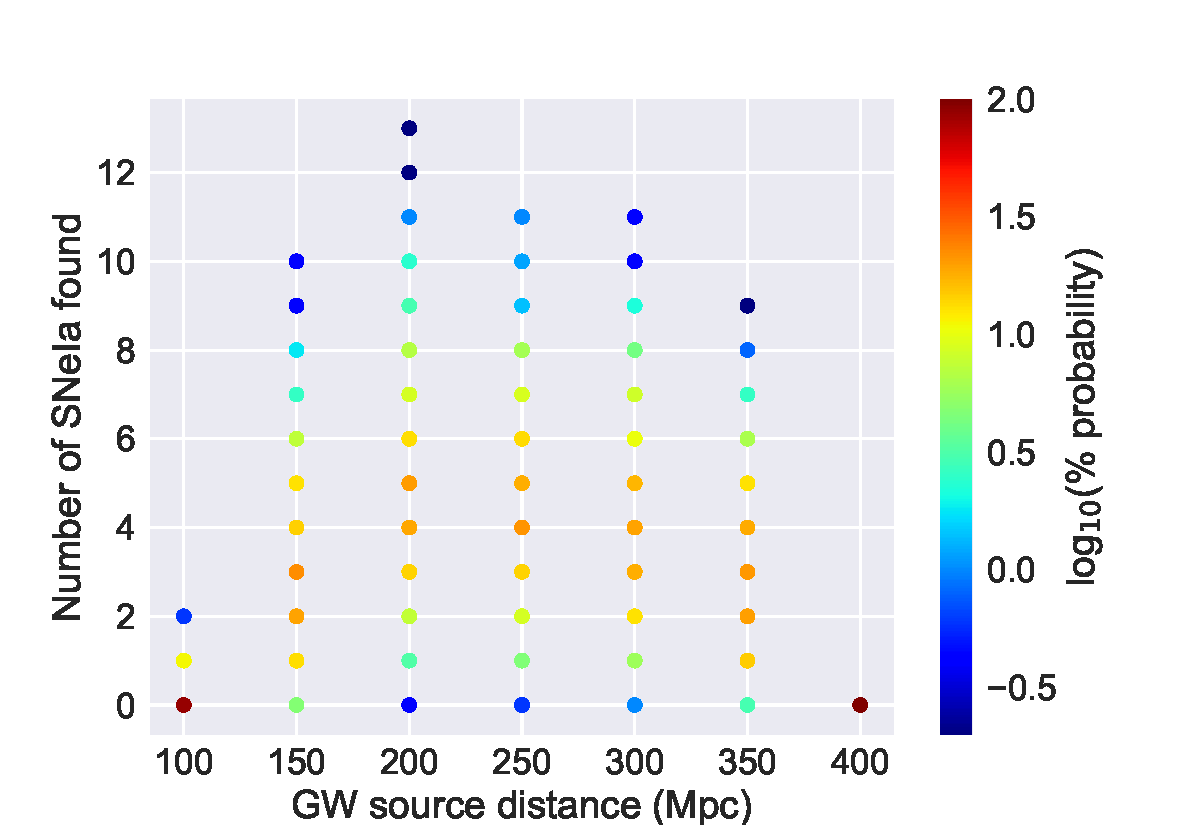
\includegraphics[width=\linewidth]{../Figs/SNIa_lim22mag_v2}
\caption{The probability of finding a given number of SNe Ia (that are likely to be confused with a kilonova), as a function of distance. We assume a survey with a four night cadence reaching $m_r\lesssim$22, a GW source localised to 30 deg$^2$, and a kilonova  $M_r=-15$.}
\label{fig:SNIa}
\end{figure}

This calculation should be taken as an approximate guide, and the exact numbers of contaminants will vary with a number of factors. Higher-cadence transient surveys, and better localisation of GW events will reduce the number of contaminants found. On the other hand, simply increasing the depth of a survey will not necessarily improve matters; while some SNe will be detected earlier (and hence ruled out) when their lightcurves are still rising, greater numbers of more distant SNe will also be detected. In any case though, it is reasonable to expect that even in the most favourable scenarios we will always have more than a single plausible candidate counterpart to any future GWs.

\subsection{A proposed strategy for EM counterpart detection}

We have demonstrated that unrelated SNe Ia will be found within the region to which a GW is localised, and that a few of these are going to appear as new sources with comparable magnitude to a potential kilonova. There are two main reasons why this is a problem. Firstly, obtaining a spectrum of a kilonova and $\sim$5 unrelated SNe Ia will take commensurately longer.
Secondly, unrelated transients make it much harder to obtain spectra of potentially rapidly fading BH-NS mergers, or of their very early ($<$1 hr) evolution. If we have five sources of comparable magnitude, and it takes $\sim1$ hr to obtain a spectrum of each, we will only obtain a spectrum of the correct candidate in $<$1~hr in a minority of cases.
The early warning from ET offers a solution to both of these problems. We propose that as soon as sufficient SNR is accumulated to localise a GW to $\sim20~\mathrm{deg}^2$ or better, we take a set of images for that region of the sky {\it before} the merger occurs.

The LSST can reach a $5\sigma$ limiting magnitude of $r\sim24.3$ with $2\times15$~s images. The readout times for each exposure will be 2~s, and as the field-of-view of LSST is $9.6~\mathrm{deg}^2$, we will likely be able to cover the entire GW footprint in a small number of pointings. Even allowing 5 minutes for slewing of the telescope, it is likely that obtaining pre-merger images will take at most 10 minutes.
After the merger, we would take a second set of images. These would be subtracted from the pre-merger template images taken $\lesssim1$ hr before; and the kilonova should be the only thing that has changed over this brief period, making it trivial to identify.

\section{Summary}

We have shown that Einstein Telescope will provide $\sim$~hr early warning of BNS mergers,
and in a substantial fraction of cases will localise these to better than $100~\mathrm{deg}^2$.
This warning provides sufficient time to trigger observations of the region with wide-field
optical telescopes, {\it immediately prior} to the merger. These images can then be used as templates
to compare a second set of post-merger images, allowing for the rapid identification of any possible
EM counterpart, {\it without} the need for costly spectroscopic screening. In addition, this technique allows for 
counterparts to be found faster, which may be essential to follow up the most rapidly fading sources.

%As a final point, we note that this strategy (obtaining templates immediately prior to a merger) could be modified to work 
%Could this be done now - much larger region and with no early warning - just look for a rising LC?


\begin{acknowledgements}
 S.~A. acknowledges support by the EU H2020 under ERC Starting Grant, no.~BinGraSp-714626.
 MF is supported by a Royal Society - Science Foundation Ireland University Research Fellowship.
\end{acknowledgements}


\bibliographystyle{aa}
\bibliography{GWbib}

\end{document}
